\chapter{Propuesta}\label{chapter:proposal}

% Introducción a Deep Learning, Neural Networks: Tipos de aprendizaje, esquema de minimización.
% Explicaciones de los modelos usados: Funciones de activacion, Relu, softmax
% Explicaciones de los modelos usados: Funciones de error, categorical crossentropy
% Explicaciones de los modelos usados: LSTM, CRF, CNN, ResNet, DenseLayer, GloVe, Attention
% Explicaciones de los modelos usados: Optimizadores Adam, Stocastic Gradient Descent, Diferenciacion automática

% Explicación del pipeline: Primero segmentación, luego link prediction
% Modelo de segmentación descrito a fondo
% Modelo de link prediction descrito a fondo

\section{Aprendizaje de Máquina}

% Hablar de problemas de regresión y de clasificación (binario y multi-class)

Aprendizaje de Máquina es una rama de la Inteligencia Artificial en la que se estudia la habilidad de 

\subsection{Overfitting y como combatirlo}

Dropout, regularizaciones, normalizaciones

\subsection{Descenso por gradiente}

Algoritmo general, Optimizadores (Adams, Stocastic Gradient Descent, Exponential Decay)

\subsection{Dense Layers}

\subsection{RNN}

Definicion de RNN, LSTM, Ventajas de RNN en secuencias

\subsection{CNN}

Definicion de CNN, [Average, Max, ...] Pooling, Ventajas de CNN en secuencias

\subsection{CRF}

Definicion de CRF, qué modela, Ventajas de CRF en secuencias

\subsection{Residual Networks}

Definicion, por qué su uso.

\subsection{Attention}

Definicion, qué hace, uso en secuencias

\subsection{Word Embeddings}

\subsection{Procesamiento de Secuencias}

Modelos sequence to sequence

\subsection{Ensemble Learning}

\section{Métricas}

% Que son las metricas y para que se utilizan. 
% Decir metricas existentes para problemas de clasificacion
% Explicar en que consisten estas metricas
% Poner ejemplos de metricas usadas como funciones de error

% \cite{grandini2020metrics}

En Aprendizaje de Máquina los modelos necesitan maneras de expresar qué tan buenos son 
en las tareas encomendadas. Para esto se crean funciones que evalúan los resultados obtenidos
por dichos modelos, estas funciones se les da el nombre de métricas. Existen diferentes tipos de
métricas para tratar con diferentes tipos de problemas. En aprendizaje supervisado una métrica se
define como una función $m_s(Y, \hat{Y})$ donde $Y$ son las predicciones verdaderas y $\hat{Y}$ son las predicciones
hechas por el modelo. En algoritmos de aprendizaje no supervisado como K-Means, K-NN son usadas funciones $m_{ns}(\hat{Y})$
donde $\hat{Y}$ son las predicciones finales. En comparación con su versión supervisada estas funciones no tiene acceso
a las predicciones verdaderas del problema.

\subsection{Regresión}

En problemas de regresión se emplean comúnmente
métricas como error medio cuadrático (MSE por sus siglas en inglés \emph{Mean Squared Error})\ref{metric:MSE}, 
raíz de MSE (RMSE por sus siglas en inglés \emph{Root Mean Squared Error})\ref{metric:RMSE},
error medio absoluto (MAE por sus siglas en inglés \emph{Mean Absolute Error})\ref{MAE} y error absoluto promedio porcentual 
(MAPE por sus siglas en inglés \emph{Mean Absolute Percentage Error}) [\cite{botchkarev2019new}].

\begin{equation}\label{metric:MSE}
	mse(Y, \hat{Y}) = \frac{1}{N} \sum^{N}_{i=1} (Y_i - \hat{Y}_i)^2
\end{equation}\caption{MSE}

\begin{equation}\label{metric:RMSE}
	rmse(Y, \hat{Y}) = \sqrt{mse(Y, \hat{Y})}
\end{equation}\caption{RMSE}

\begin{equation}\label{metric:MAE}
	mae(Y, \hat{Y}) = \frac{1}{N} \sum^{N}_{i=1} |Y_i - \hat{Y}_i|
\end{equation}\caption{MAE}

\begin{equation}\label{metric:MAPE}
	mape(Y, \hat{Y}) = \frac{1}{N} \sum^{N}_{i=1} |\frac{Y_i - \hat{Y}_i}{Y_i}|
\end{equation}\caption{MAPE}

\subsection{Clasificación}

En problemas de clasificación son empleadas otras medidas que toman en cuenta la naturaleza discreta del problema. 
Medidas como precisión, recobrado, certeza (accuracy en inglés) y F1 son utilizadas principalmente en la 
evaluación de los resultados, mientras que para evaluar la pérdida se usa entropía cruzada 
(\emph{cross entropy} en inglés).

\subsubsection{Matriz de confusión}

La matriz de confusión es una via de representar los resultados de dos clasificadores. Esta matriz en $M_{ij}$ 
indica la cantidad de elementos que clasificó como clase $i$ el primer clasificador y
como clase $j$ el segundo clasificador. En su uso práctico
un clasificador son las etiquetas verdaderas mientras que el otro es el clasiificador que se está evaluando. 
En problemas de la clasificación binaria, donde se busca saber si existe pertenencia o no de un elemento a una clase,
se pueden observar los siguientes casos.

\begin{itemize}
	\item Verdaderos Positivos (VP): Elementos clasificados correctamente que pertenecen a la clase.
	\item Verdaderos Negativos (VN): Elementos clasificados correctamente que no pertenecen a la clase.
	\item Falsos Positivos (FP): Elementos clasificados incorrectamente que pertenecen a la clase.
	\item Falsos Negativos (FN): Elementos clasificados incorrectamente que no pertenecen a la clase.
\end{itemize}

TODO FOTO DE MATRIZ DE CONFUSION BINARIA

\subsubsection{Precisión}

La precisión es la medida que indica la probabilidad de que la clasificación de una clase sea correcta. Esto 
se puede observar como la proporción de los elementos correctamente clasificados sobre el total de 
elementos clasificados:

\begin{equation}
	prec_i = \frac{VP}{VP + FP}
\end{equation}

En problemas de clasificación múltiple surge la versión macro de esta medida calculada como la media de todas
las precisiones de las clases existentes:

\begin{equation}
	prec_{macro} = \sum^K_{i=1} \frac{prec_i}{K}
\end{equation}

\subsubsection{Recobrado}

El recobrado es la medida que indica la probabilidad de que se clasifique correctamente un elemento de la clase
del total existente. Esto se puede observar como la proporción de los elementos correctamente clasificados sobre el 
total de elementos que pertenecen a la clase:

\begin{equation}
	rec_i = \frac{VP}{VP + FN}
\end{equation}

En problemas de clasificación múltiple surge la versión macro de esta medida calculada como la media de todos
los recobrados de las clases existentes:

\begin{equation}
	rec_{macro} = \sum^K_{i=1} \frac{rec_i}{K}
\end{equation}

\subsubsection{F1}

La medida F1 es la media armónica de la precisión y el recobrado. En esta la contribución de la precisión y el
recobrado al resultado final es el mismo, aunque es posible buscar variaciones de acuerdo a al problema a tratar:

\begin{equation}
	f1_i = 2 (\frac{prec_i * rec_i}{prec_i + rec_i})
\end{equation}

En problemas de clasificación múltiple surge la versión macro de esta medida calculada la propia medida F1 pero
utilizando la precisión y recobrado macro del problema:

\begin{equation}
	f1_{macro} = 2 (\frac{prec_{macro} * rec_{macro}}{prec_{macro} + rec_{macro}})
\end{equation}

\subsubsection{Entropía cruzada}

Esta medida se encarga de evaluar qué tan diferentes son dos funciones de distribución $p$ y $q$, por lo que
pequeños valores de esta indican mayor similitud. En su versión discreta se formula:

\begin{equation}
	H(p, q) = - \sum_{x \in D} p(x) \log q(x)
\end{equation}

\section{Modelo Propuesto}

El modelo propuesto se divide en dos secciones. En la primera sección se realiza la segmentación y clasificación de 
las UDAs como tareas conjuntas. En la segunda sección se realizará la predicción de enlaces y su clasificación, tomando
como tareas auxiliares la clasificación de las UDA. En dependencia de los resultados obtenidos, la clasificación final de 
las UDAs se escoge de la mejor sección (TODO IMPLEMENTAR ESTO, O NO). 

\subsection{Segmentación y clasificacón de UDAs}

Esta primera parte se modeló como un problema secuencia a secuencia cuyo objetivo es convertir la secuencias de 
tokens en secuencias de etiquetas BIOES con sus respectivas clasificaciones. Además de las 
anotaciones BIOES se agrega información extra sobre el tipo de UDA al que pertenece el segmento.

\subsubsection{Modelo}

Sea $D$ un documento, este es separado en una secuencia de $n$ tokens $D_i$ donde $n$ es la mayor longitud encontrada
en los documentos del conjunto de datos. A cada token se le es asignado
su representación vectorial \textbf{GloVe} de dimensión $g$ dando como resultado $G_{ij} \in \mathbb{R}^{n \times g}$.
Esta representación inicial presenta información semántica de las palabras además que conserva las relaciones 
espaciales entre ellas. 

Para la representación de información morfológica de la palabra se construyen dos
codificadores que procesan los caracteres de cada token y devuelven una representación vectorial de estos.
A cada caracter se le es asignado un vector que será entrenado convirtiendo un token en un vector de dimensión
$q \times c$ donde $q$ es el tamaño máximo de palabra en el conjunto de datos y $c$ es la dimensión del vector
asignado a cada caracter.

Uno de estos modelos está basado en \textbf{CNN}, este modelo entrena una representación de caracteres de dimensión
$cd$ representando un token como un vector de dimensión $q \times cd$. Se conforma por una capa de convolución unidimensional
con $f$ filtros y un kernel de tamaño $k$ seguida por un \textbf{Max Pool Layer} que convierte la secuencia en un vector
de dimensión $1 \times f$ que luego este vector es concatenado a la representación del token a que pertenece.

Otro modelo utilizado para calcular una representación morfológica se encuentra basado en \textbf{RNN}. Se usó
un modelo LSTM bidireccional con dimensión $l$ para calcular la representación del token, para las dimensiones de los caracteres se
utilizan vectores de tamaño $l$, el resultado final constituye la concatenación de la corrida hacia adelante y la corrida
hacia atrás formando una representación de dimensión $1 \times 2l$ del token. Este vector es concatenado a la representación
del token correspondiente.

Otro atributo usado en la representación de los tokens constituyen las etiquetas de Partes de la Oración de estos.
El conjunto de etiquetas elegido es un conjunto universal [TODO \cite{Referencia a la def}] aplicable a cualquier idioma.
De estas etiquetas se les extraen la codificación one-hot y esta es transformada por una cada densa con $p$ neuronas
y función de activación \textbf{relu}, el resultado es concatenado a la representación del token correspondiente.

Del proceso de vectorización sale un vector con dimensión $n \times t$ donde $t$ es la dimensión final de la representación
de los tokens. Este vector es modificado por una capa \textbf{LSTM} bidireccional de dimensión $m$, a esta salida se le 
añade una conexión residual al ajustarle la dimensión con una capa densa. Luego la secuencia es procesada por una 
capa densa de dimensión $k$ produciendo una representación final de dimensión $q \times k$.
Finalmente se utiliza una capa \textbf{CRF}
para la clasificación final de la secuencia en las etiquetas finales. El resultado final constituye un vector
de dimensión $q$ que representa las clasificaciones inferidas por el modelo.

\begin{figure}[h!]
	\begin{center}
		\begin{center}
			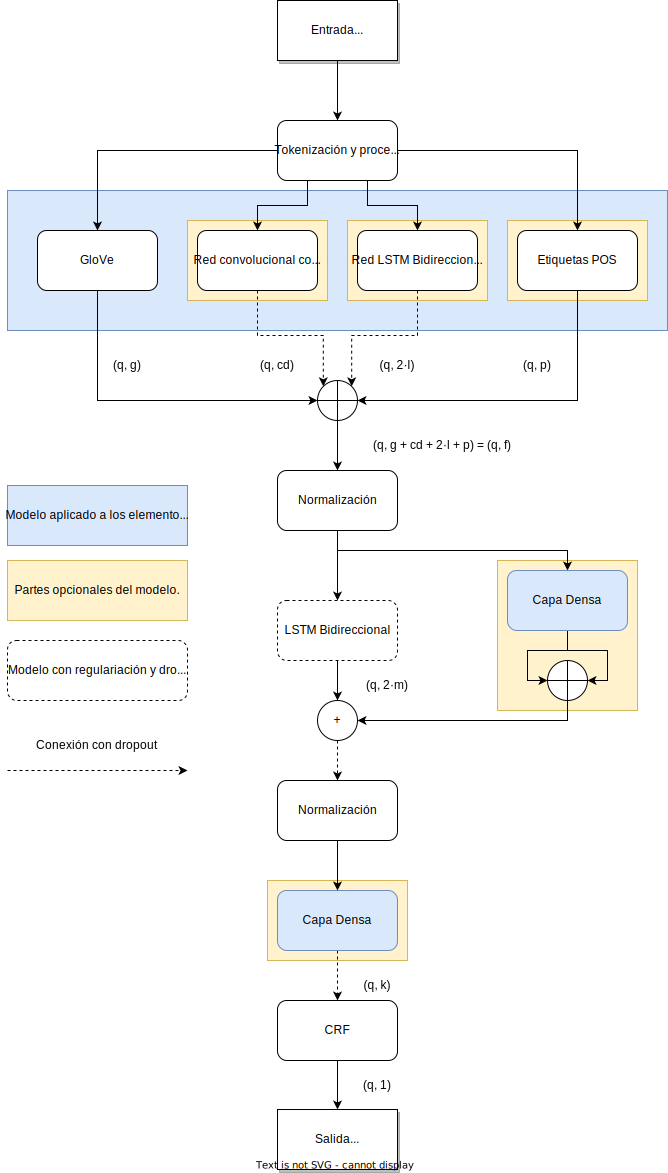
\includegraphics[scale=.3]{Graphics/Modelo Segmenter UDA.drawio.png}
            % \includesvg[options]{Graphics/Modelo Segmenter UDA.drawio.svg}
        \end{center}
	    \caption{Segmentador UDAs}\label{fig:seg_uda}
	\end{center}
\end{figure}

Debido a la escasez de los datos se tuvieron que tomar medidas para prevenir el overfitting. Entre cada capa de 
procesamiento se añadieron capas de normalización y dropout con un porciento de $d$\%. Además de esto se 
las capas de \textbf{LSTM} se utilizaron regularizaciones L2. Como optimizador se utilizó Adam.

\subsubsection{Posporcesamiento}

La salida del modelo constituye una secuencia de etiquetas en formato BIOES. La secuencia devuelta puede que contenga
errores en la estructura BIOES, por ejemplo, secuencias no terminando en E, segmentos continuos con más de una meta-etiqueta.
Para la corrección de la estructura se propone el siguiente algoritmo, el cual se divide en dos partes. La primera
parte consiste en arreglar la estructura BIOES, para esto se mantiene una ventana de tamaño
3 sobre la secuencia y asume que la parte anterior a la posición de la ventana no presenta errores, al encontrar una
ventana inválida se necesita observar la siguiente ventana para poder decidir cómo se arregla el error ya que se
podría dar el caso de OOI OIO, en donde solamente viendo la primera ventana no se podría saber si el cambio 
correcto corresponde a sustituir I por B o por S. Una vez observado las dos ventanas se procede a realizar el 
arreglo correspondiente. Una vez se tiene la secuencia tiene la estructura BIOES correctamente anotada el problema
consiste en arreglar las meta-etiquetas, ya que una misma secuencia BIOES pudo haber sido anotada con diferentes
tipos de meta-etiquetas, en este caso se toma la etiqueta más representativa de la secuencia. Este procedimiento
devuelve una secuencia BIOES correctamente anotada.

\subsection{Predicción de enlaces}

Este modelo consiste en dados dos pares de UDA previamente extraías y su distancia argumentativa, 
extraer y clasificar la relación entre ellas. Como tarea auxiliar se realiza además la clasificación 
de las UDAs.

\subsubsection{Modelo}

Sea dos UDAs, $S$ y $T$, una representa la fuente de la relación, mientras que la otra representa
el objetivo. Estas secuencias son tokenizadas y se les asigna la representación GloVe de cada palabra, obteniendo
dos vectores de dimensión $u \times g$, donde $u$ es el tamaño máximo de UDAs en el conjunto de entrenamiento.
Estos vectores son modificados por una red densa compuesta por $ca$ capas con activación relu. 
Al finalizar este procesamiento se añade una conexión residual
a la salida. El próximo paso consiste en aplicar una capa densa de dimensión $di$ y luego un \emph{average pooling}
de tamaño $dp$. El objetivo del procesamiento anterior consiste
en la reducción de dimensionalidad de la entrada, al final se obtiene vectores de dimensión $\frac{q}{di}, dq$. 
Estos vectores son modificados por un LSTM bidireccional con $lm$ unidades. Un módulo de atención es aplicado, 
en este actúan como consultas el promedio de los vectores objetivo y como llaves y valores los vectores fuentes,
este procedimiento es simétrico para el procesamiento de los vectores objetivo.
La salida de los procesamientos son concatenados con la distancia argumentativa obteniendo una representación 
conjunta de la relación a analizar. Esta representación conjunta es modificada por una red residual obteniendo
una representación final de dimensión $ff$ y luego sometida a los clasificadores de relación y de tipos de UDAs.

\begin{figure}[h!]
	\begin{center}
		\begin{center}
			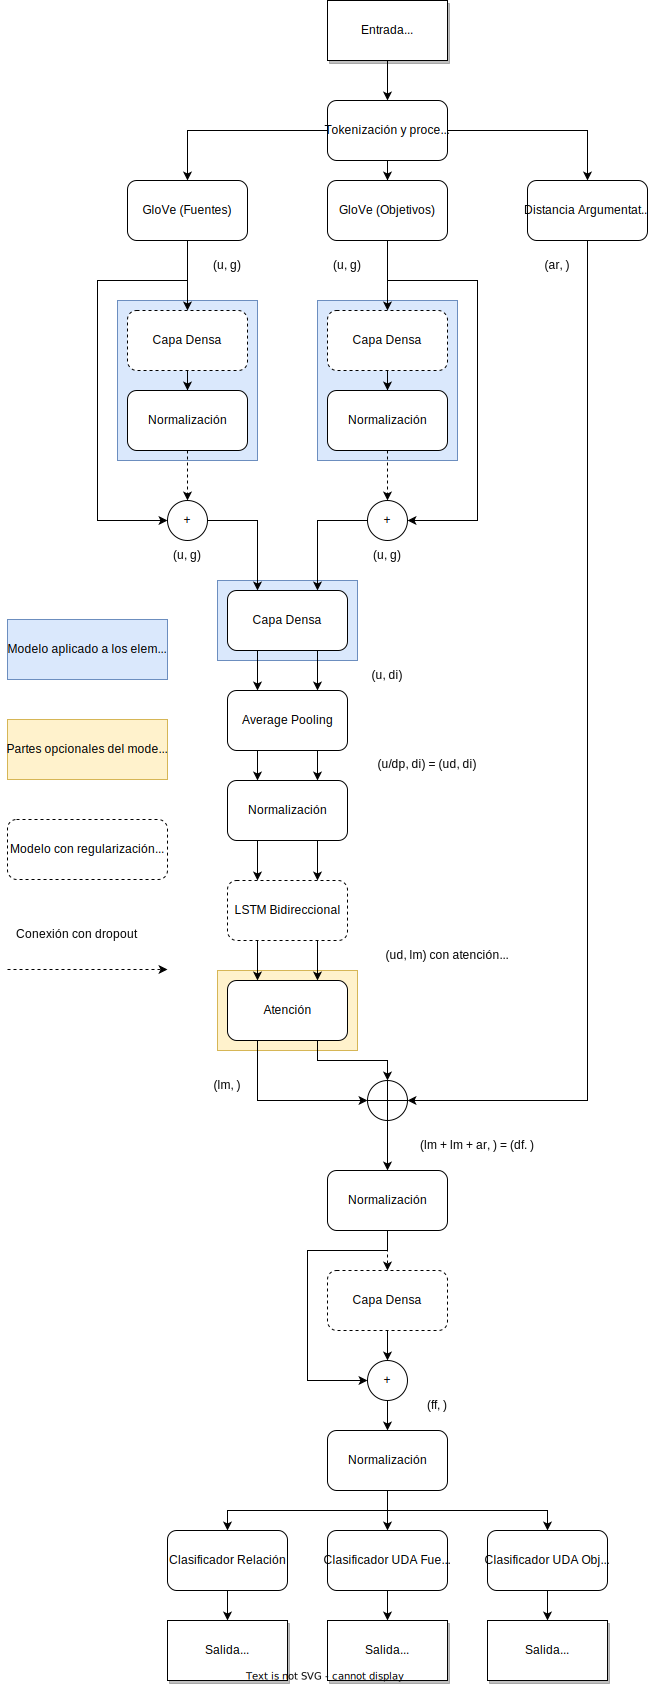
\includegraphics[scale=.3]{Graphics/Modelo Link Prediction.drawio.png}
            % \includesvg[options]{Graphics/Modelo Link Prediction.drawio.svg}
        \end{center}
	    \caption{Predictor de enlaces}\label{fig:link_predictor}
	\end{center}
\end{figure}

Para prevenir el overfitting se agregaron capas de normalización y de dropout entre cada proceso y se usó regularizaciones
L2 en las capas densas y LSTM. Como optimizador se utilizó Adam con descenso exponencial.

